\documentclass[12pt]{article}
\usepackage{amsmath}
\usepackage{amsthm}
\usepackage{amssymb}
\usepackage{bbold}
\usepackage{bm}
\usepackage{graphicx}
\usepackage{float}
\usepackage[parfill]{parskip}
\usepackage{subcaption}
\usepackage[a4paper, portrait, margin=1in]{geometry}

\begin{document}

\title{Spatial-temporal Modeling of Ambient Ozone}
\author{Lucy Lu, Sam Yin}
\date{May 2, 2017}
\maketitle

\section{Introduction \& Data Description}
The objective of this project is to build space-time models to forecast next-hour ground-level ozone concentrations at various locations across the U.S.. 

\begin{figure}[H]
\centering
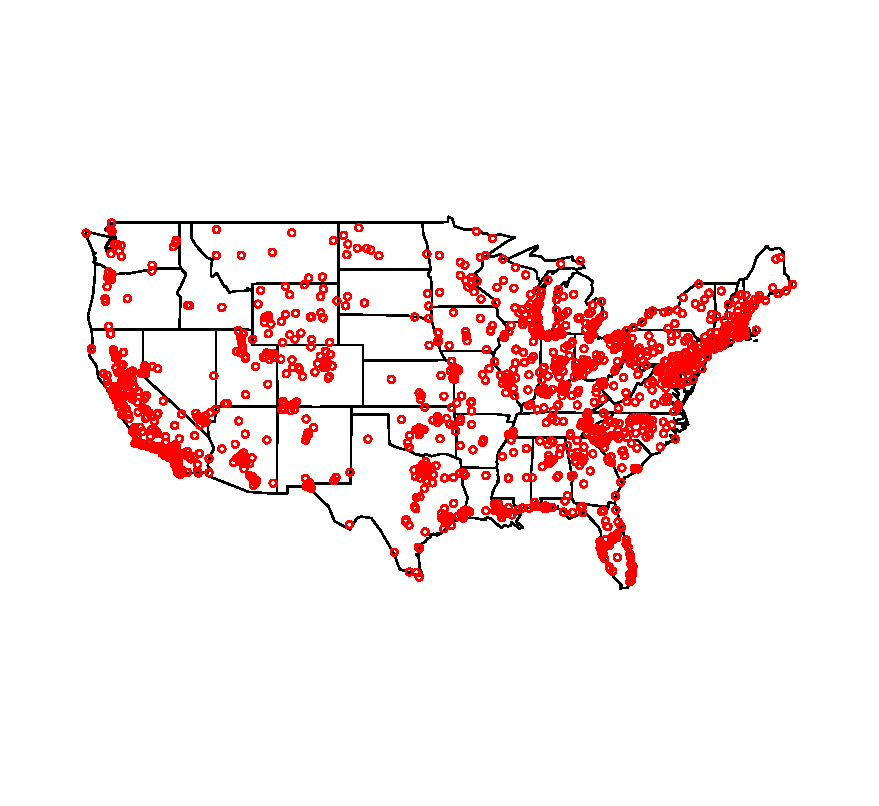
\includegraphics[scale = 0.4]{site_map.eps}
\caption{Map of ozone sites across the U.S.}
\end{figure}

Hourly ozones were collected at 1249 sites across the U.S. from 06/01/2015 00:00:00 to 06/30/2015 23:00:00. Overall, there is about 9\% missing data. Considering missing data are more common at some sites than at others, we decided to use data only from sites where completeness is at least 95\%. This leaves us with 935 sites. To account for missing data at the remaining sites, we take the average of the two observed data points closest to the missing data point. Since space-time models are inherently computing-intensive, to ensure our models are feasible in practice, we choose to divide the U.S. into 25 subregions (5 by 5 grid) and model by region. In this project, we only illustrate the modeling of region 1 (New England area, 71 sites). The hope is that with a multi-core machine, we can model the regions in parallel, and thus reducing run-time to an affordable range. 

\begin{figure}[H]
\centering
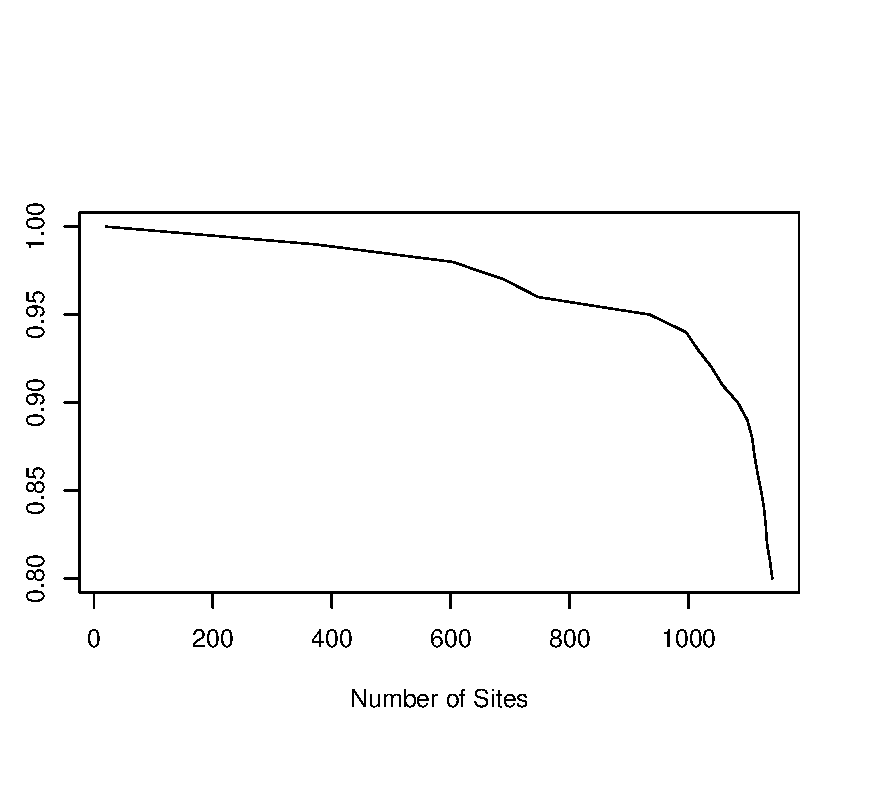
\includegraphics[scale = 0.4]{completeness_by_n_sites.eps}
\caption{Cut-off percentage of completeness by number of sites}
\end{figure}

\section{EDA}
From Figure 3, we can see that the running plot of average ozone (over all sites in region 1) is approximately stationary with no apparent trend. Its PACF shows strong autocorrelations in the first two lags and quickly diminishes, providing evidence for including up to two autoregressive terms. Its ACF displays an oscillating pattern with a peak at the $24^{\text{th}}$. This signals the potential for including a day-long seasonality term. 

\begin{figure}[H]
\centering
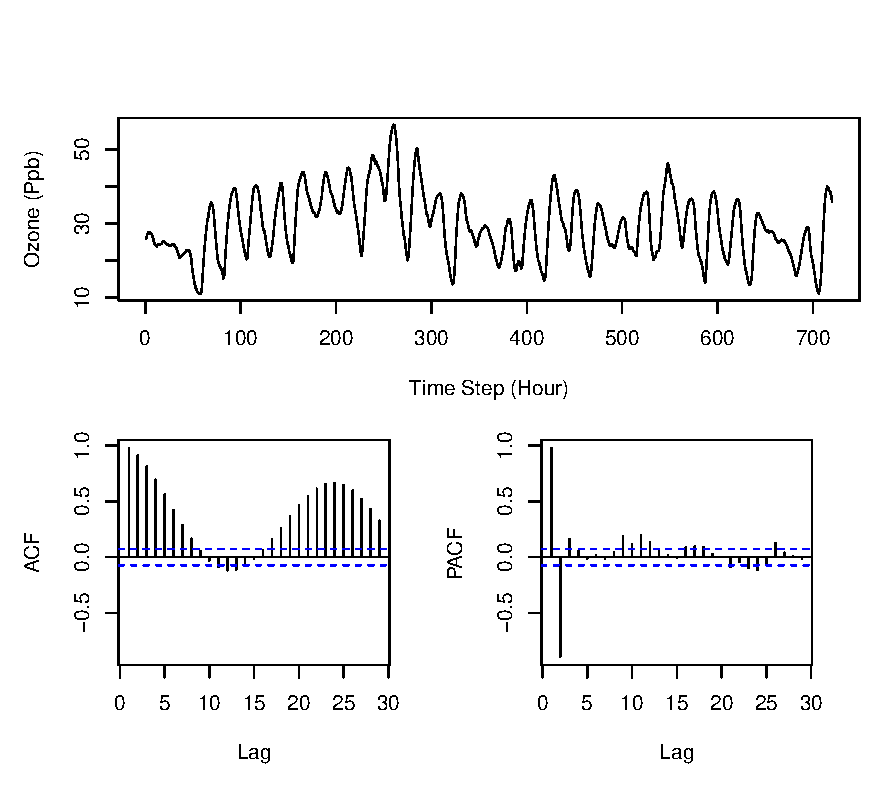
\includegraphics[scale = 0.4]{ts_o3.eps}
\caption{Time series display of average ozone concentration (of all sites) in region 1}
\end{figure}

Except for one outlier, the semivariogram of average ozone (over all time points) justifies the exponential covariance structure, i.e. the semivariogram increases as the distance between two sites increases, and it approaches an upper limit as the distance approaches infinity (Figrue 4). From visual inspection, we can estimate that the nugget is around 5, the sill is around 20, and the range is around 1.5.

\begin{figure}[H]
\centering
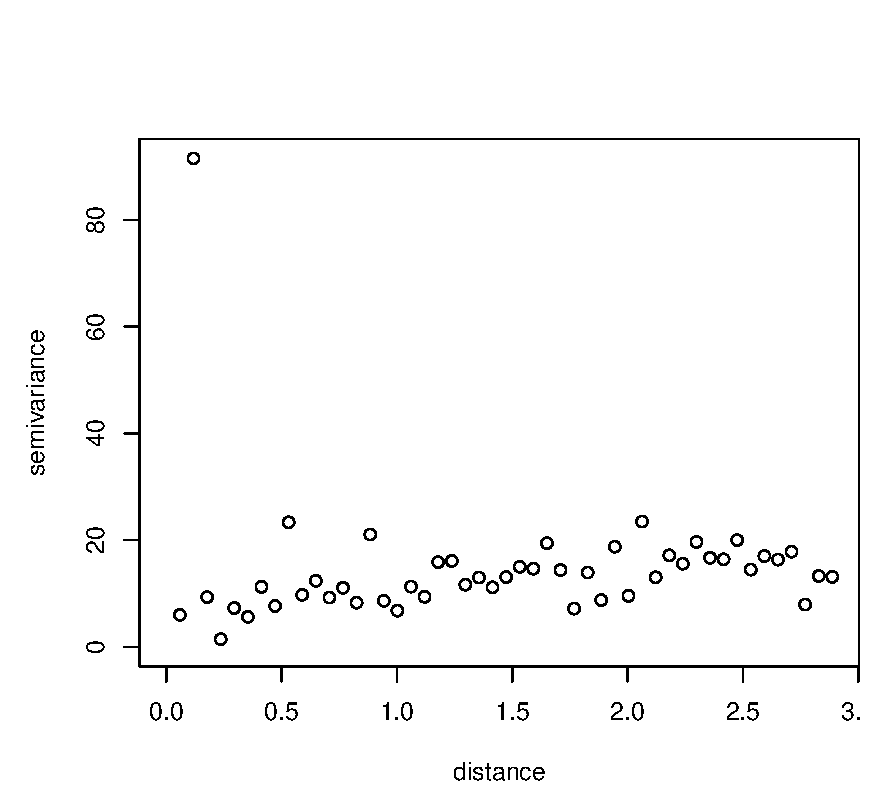
\includegraphics[scale = 0.4]{variogram.eps}
\caption{Semivariogram of average ozone concentration (of all time points) in region 1}
\end{figure}

\section{Modeling}
Ideally, spatiotemporal modeling should consider shared information between space and time by specifying the covariance structure among observations at all locations and all time points $cov(y_{s, t}, y_{s^{\prime}, t^{\prime}})$ in terms of both spatial distance $||s - s^{\prime}||$ and temporal lag $|t - t^{\prime}|$ (assuming discrete time). The flexibility of this approach poses two main challenges. The first one is how to determine the weight assigned to spatial and temporal dimensions (and potentially their interaction). Specifically, if we assume a covariance structure of the form $\phi_1 \exp(-\phi_2 * d ^ \nu)$, there are infinitely many ways to incorporate spatial distance and temporal lag in the parametrization. Another issue is computation. Since the Gaussian Process component of the model induces sampling from (conditional) multivariate normal distribution, the inversion and multiplication of covariance matrix become the primary constraint of computational efficiency. As the number of time points and locations increases, the dimension of covariance matrix grows with $O(n^2)$, which significantly slows down model fitting.

For simplicity, in this analysis we assume separation of spatial and temporal dimensions and construct the following additive model: 

\begin{align}
y(s, t) &= w(s, t) + e(s, t) \\
&= \alpha(t) + \omega(s) + \epsilon(s, t).
\end{align}

In other words, $\alpha(t)$ is constant to all sites at a given time point $t$, and $\omega(s)$ is constant at all time points given a specific site $s$. 

\begin{enumerate}
\item AR(1): $\alpha(t) = \delta + \phi \alpha(t - 1)$ 
\item MA(1): $\alpha(t) = \delta + w_t + \theta w_{t - 1},\ w_{1:T} \overset{\text{i.i.d.}}{\sim} N(0, \sigma_w^2)$
\end{enumerate}

Two choices of the temporal structure $\alpha(t)$, $AR(1)$ and $MA(1)$, are compared in their performance of fitting and kriging. 

\begin{equation}
\omega(\tilde{s}) \sim \mbox{MVN}(\mathbf{0}, \bm{\Sigma}_{\omega})
\end{equation}
where $\{\bm{\Sigma}_{\omega}\}_{ij} = \sigma_\omega^2 \exp(-\phi_{\omega}||s_i - s_j||_2)$ for $i \neq j$ \\
\begin{equation}
\epsilon(s, t) \sim N(0, \sigma_\epsilon^2)
\end{equation}

$\omega(s)$ is a Gaussian process model with exponential covariance, and $\epsilon(s, t)$ is a normal random error. 

The parameters of time series module and Gaussian process are trained jointly with JAGS 4.2.0 in R. 4,000 iterations were used, with 3,000 burn-ins and 3 parallel chains. Ideally, we would like to use a 120-hour training window for every next-hour forecast, and shift the window one hour forward as forecasting goes on. Here, we only demonstrate results of the first forecast (using the first 120 hour as the training window to forecast the $121^{th}$ hour ozones at different sites). We randomly selected 47 sites for in-sample forecasting, and left the other 24 sites for out-of-sample forecasting (kriging). 

Forecasting involves two stages: (i) in-sample forecasting is achieved by sampling from the posterior distribution of time series model parameters ($\phi$ or $\theta$; $w_t$) to generate the next time point estimate $\hat{y}_{t + 1}$ (mean structure); (ii) kriging is achieved by sampling from the conditional multivariate normal distribution with the covariance structure specified by GP parameters ($\sigma_{\omega}^2$, $\phi_{\omega}$) sampled from posterior distribution.
\begin{align}
\mathbf{Y}|\mathbf{X} \sim \mbox{MVN}(\bm{\mu}_{\mathbf{Y}} + \bm{\Sigma}_{YX}\bm{\Sigma}_{X}^{-1}(\mathbf{X} - \bm{\mu}_{\mathbf{X}}), \bm{\Sigma}_{Y} - \bm{\Sigma}_{YX}\bm{\Sigma}_{X}^{-1}\bm{\Sigma}_{XY})
\end{align}

The model evaluation consists of in-sample and out-of-sample predictive performance. Notice that the out-of-sample forecasting is based on the fitted values of sites in the training set, therefore the performance of in-sample forecasting largely determines the kriging accuracy. We used predictive mean squared error (PMSE), average 95\% credible interval lengths, 95\% empirical coverage, and continuous rank probability score (CRPS) for evaluation. Criteria arise by averaging over all sites and all time points.

\begin{align*}
\text{PMSE} &= \frac{\sum_{t = 1}^m\sum_{s = 1}^{n}(\hat{y}(s, t) - y_{obs}(s, t))^2}{mn} \\
\text{Average Interval Length} &= \frac{\sum_{t = 1}^{m}\sum_{s = 1}^{n}\text{Length of 95\% CI at Time $t$ Site $s$}}{mn} \\
\text{Coverage} &= \frac{\sum_{t = 1}^{m}\sum_{s = 1}^{n}\mathbf{1}(y_{obs}(s, t) \in 95\% CI)}{mn} \\
\text{CRPS} &= E_{F}|y(s, t) - y_{obs}(s, t)| - \frac{1}{2}E_{F}|y(s, t) - y'(s, t)|
\end{align*}


\section{Results}
According to the summary of predictive performance, the AR(1) model is doing better than the MA(1) model at in-sample forecasting (Table 1), with lower PMSE and lower CRPS. However, the situation is reversed for out-of-sample forecasting, where the MA(1) model produced lower PMSE and lower CRPS than the AR(1) model (Tabel 2). The predicted by observed ozone plots show that the AR(1) model has almost no predictive power at kriging sites (Figure 5). Curiously, despite a strong out-of-sample predictive performance, the MA(1) model has almost no power forecasting in-sample. One explanation could be that the temporal structures have strong locality that is not accounted for by the naive additive specification. Moreover, the parameter estimates of the AR(1) model generally agree with the PACF and the semivariogram showed earlier, whereas the MA(1) model overestimated the nugget and sill by a large margin (Table 3). This may partially explain its wider intervals and worse performance for in-sample forecasting. 

\begin{table}[H]
\centering
\begin{tabular}{|c c c c c|}
\hline
Model & PMSE & Interval & Coverage & CRPS \\\hline 
AR(1) & 17.7 & 12.98 & 0.85 & 2.36\\
MA(1) & 126.24 & 36.56 & 0.91 & 6.56 \\\hline
\end{tabular}
\caption{Summary of predictive performance at fitting sites (47)}
\end{table}

\begin{table}[H]
\centering
\begin{tabular}{|c c c c c|}
\hline
Model & PMSE & Interval & Coverage & CRPS \\\hline 
AR(1) & 60.08 & 12.84 & 0.79 & 4.29\\
MA(1) & 38.00 & 27.49 & 0.92 & 3.45 \\\hline
\end{tabular}
\caption{Summary of predictive performance at kriging sites (24)}
\end{table}

\begin{table}[H]
\centering
\begin{tabular}{|c c c|c c c|}
\hline
AR(1) & Mean & 95\% CI & MA(1) & Mean & 95\% CI \\\hline
$\sigma_\omega^2$ & 4.32 & (3.59, 5.20) & $\sigma_\omega^2$ & 49.97 & (44.95, 55.55) \\
$\phi_\omega$ & 0.15 & (0.10, 0.20) & $\phi_\omega$ & 0.57 & (0.48, 0.67) \\
\hline
$\phi$ & 0.88 & (0.87, 0.89) & $\theta$ & 1.06 & (0.76, 1.44) \\
$\delta$ & 3.83 & (2.80, 5.14) & $\sigma_w^2$ & 13.26 & (7.76, 20.21) \\
$\sigma_\epsilon^2$ & 6.40 & (6.07, 6.75) & $\delta$ & 25.51 & (24.11, 26.94) \\
 &  &  & $\sigma_\epsilon^2$ & 14.68 & (13.00, 16.41) \\
\hline
\end{tabular}
\caption{Summary of parameter posterior distributions}
\end{table}

\begin{figure}[H]
\centering
\begin{subfigure}{.5\textwidth}
	\centering
	\includegraphics[scale = 0.4]{pred_in_ar.eps}
	\caption{}
\end{subfigure}%
\begin{subfigure}{.5\textwidth}
	\centering
	\includegraphics[scale = 0.4]{pred_out_ar.eps}
	\caption{}
\end{subfigure}
\caption{Pedicted vs observed ozones, AR(1)}
\end{figure}

\begin{figure}[H]
\centering
\begin{subfigure}{.5\textwidth}
	\centering
	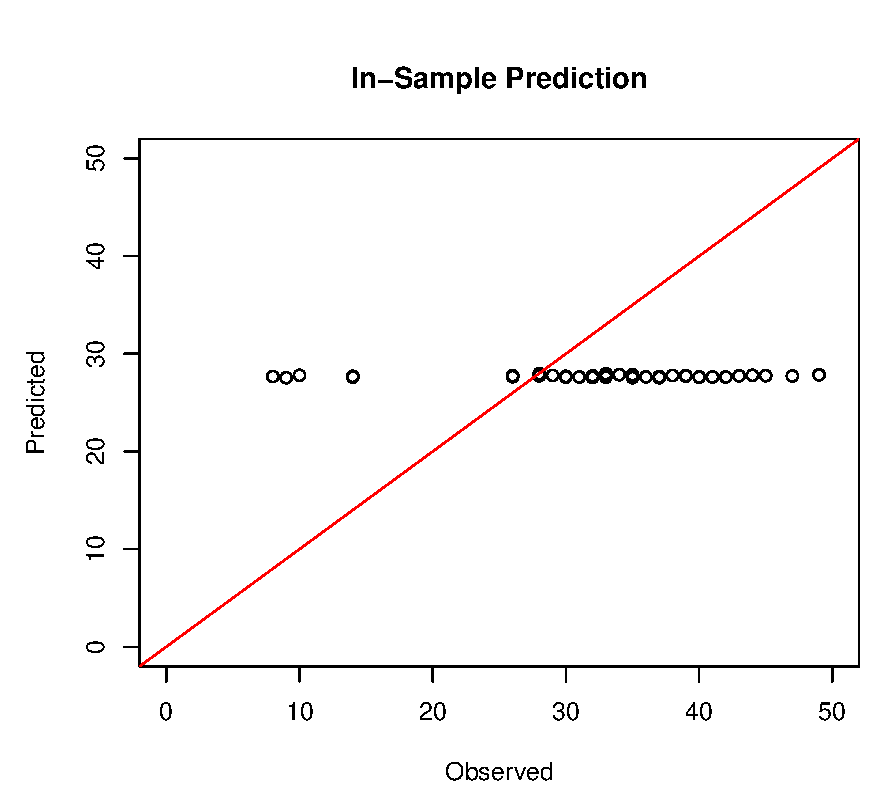
\includegraphics[scale = 0.4]{pred_in_ma.eps}
	\caption{}
\end{subfigure}%
\begin{subfigure}{.5\textwidth}
	\centering
	\includegraphics[scale = 0.4]{pred_out_ma.eps}
	\caption{}
\end{subfigure}
\caption{Pedicted vs observed ozones, MA(1)}
\end{figure}

\section{Discussion}

% \subsection{In-Sample vs. Out-of-Sample Forecasting}
% The model evaluation consists of fitting and kriging performance. Both forecasting involve two stages: (i) sample from the posterior distribution of time series model parameters ($\phi$ or $\theta$; $w_t$) to generate the next time point estimate $\hat{y}_{t + 1}$ (mean structure); (ii) sample from the conditional multivariate normal distribution with the covariance structure specified by GP parameters ($\sigma_{\omega}^2$, $\phi_{\omega}$) sampled from posterior distribution.
% \begin{align}
% \mathbf{Y}|\mathbf{X} \sim \mbox{MVN}(\bm{\mu}_{\mathbf{Y}} + \bm{\Sigma}_{YX}\bm{\Sigma}_{X}^{-1}(\mathbf{X} - \bm{\mu}_{\mathbf{X}}), \bm{\Sigma}_{Y} - \bm{\Sigma}_{YX}\bm{\Sigma}_{X}^{-1}\bm{\Sigma}_{XY})
% \end{align}
% Notice that the out-of-sample forecasting is based on the fitted values of sites in the training set, therefore the performance of in-sample forecasting largely determines the kriging accuracy.

\subsection{Time Series Model}
In this analysis only two simple time series models, $AR(1)$ and $MA(1)$ are compared. Under the additive assumption, we could analyze the change of ground-level ozone concentration over time using the average of all sites. However, in reality the temporal pattern of ozone concentration is nearly intractable from observations without prior knowledge of spatial correlation, and averaging or pooling over the spatial dimension could bias the estimation of temporal factor. A grid search of Autoregressive integrated Moving Average (ARIMA) model parameters ($p, q, d$) with AIC/BIC or prediction accuracy criteria will potentially identify a better time series model. The time series also demonstrate seasonality with a period of approximately 24 hours. Seasonality is not incorporated in the aforementioned model due to complexity in parametrization.

\subsection{Additive Assumption and Computational Efficiency}
The additive assumption in this analysis is limiting to a great extent. The amount of shared information between space and time is nontrivial if not essential. The downside of more flexibility in modeling is computational inefficiency, since most multivariate sampling schemes involve high-dimensional (covariance) matrix computation (approximation may be available but tend to affect performance). Alternative approaches include mixture models (assume a set of local/global basis functions which are computationally less challenging and estimate both parameters and weights) and latent space models (project time and space to a latent space/kernel space where the covariance structure is less complicated).

\section{Appendix}
\begin{verbatim}
# AR(1)
y <- t(ozone.ppb_train[, 1:120])
d <- d_train
m <- nrow(y) # time step
n <- ncol(y) # site
I <- diag(n)

jags.data <- c('y', 'd', 'm', 'n', 'I')
jags.params <- c("a0", "b1", "sig2a", "phi", "sig2e")

model <- function(){
  for (t in 2:m){
    y[t, ] ~ dmnorm(a0 + b1*y[(t - 1), ], inverse(Sigma))
  }

  for (i in 1:(n - 1)){
    for (j in (i + 1):n){
      Sigma[i, j] <- sig2a*exp(-phi*d[i, j])
      Sigma[j, i] <- Sigma[i, j]
    }
  }

  for (i in 1:n){
    Sigma[i, i] <- sig2a + sig2e
  }

  # priors
  a0 ~ dmnorm(rep(25, n), I/100)
  b1 ~ dunif(-1, 1)
  tau_a ~ dgamma(2, 2)
  sig2a <- 1/tau_a
  phi ~ dnorm(1, 0.01);T(0, )
  tau_e ~ dgamma(2, 2)
  sig2e <- 1/tau_e

}

bf.sim <- jags(data = jags.data, inits = NULL, jags.params, n.chains = 3,
               n.iter = 4000, n.burnin = 3000, n.thin = 1, model.file = model)

# MA(1)
library(rjags)
library(stringr)
get_coda_parameter <- function(coda, pattern) {
  w <- coda[[1]] %>% colnames() %>% str_detect(pattern)
  coda[[1]][, w, drop = FALSE]
}


m1_code <- "
  model{
    for (t in 1:n_t) {
      y[, t] ~ dmnorm(mu + y_t[t], inverse(Sigma_w))
    }
    
    for (i in 1:(n_s - 1)) {
      for (j in (i + 1):n_s) {
        Sigma_w[i, j] <- sigma2_w * exp(- phi * d[i, j])
        Sigma_w[j, i] <- Sigma_w[i, j]
      }
    }
    
    for (k in 1:n_s) {
      Sigma_w[k, k] <- sigma2_w + sigma2
    }
    
    for (t in 2:n_t) {
      y_t[t] <- w_t[t] + theta * w_t[t - 1]
    }
    y_t[1] <- w_t[1]
    
    for (n in 1:n_s) {
      mu[n] <- beta0
    }
    
    for (t in 1:n_t) {
      w_t[t] ~ dnorm(0, tau_0)
    }
    beta0 ~ dnorm(25, 0.01)
    sigma2_w <- 1 / tau_w; tau_w ~ dgamma(2, 2)
    sigma2 <- 1 / tau; tau ~ dgamma(2, 2)
    phi ~ dnorm(1, 0.01) T(0, )
    theta ~ dnorm(0, 1)
    sigma2_t <- 1 / tau_0; tau_0 ~ dgamma(2, 2)
  }"

m1_train <- jags.model(textConnection(m1_code), 
                       data = list(d = d_train, 
                                   n_s = nrow(ozone.ppb_train), 
                                   n_t = ncol(ozone.ppb_train), 
                                   y = ozone.ppb_train), 
                       n.adapt = 2000)

update(m1_train, n.iter = 10000)

m1_coda_train <- coda.samples(m1_train, 
                              variable.names = c("beta0", "sigma2", 
                                                 "sigma2_w", "phi", 
                                                 "theta", "sigma2_t", "w_t"), 
                              n.iter = 10000)

m1_params_train <- get_coda_parameter(m1_coda_train, 
                                      "beta0|sigma2|phi|theta|w_t")
summary(m1_params_train[, 1:6])
# prediction
m1_insample_pred <- matrix(nrow = nrow(site_train), ncol = 1000)
for (i in 1:ncol(m1_insample_pred)) {
  m1_insample_pred[, i] <- mvrnorm(n = 1, 
                                   mu = rnorm(n = nrow(m1_insample_pred), 
                                              mean = m1_params_train[i, 1] + 
                                                m1_params_train[i, 6] * 
                                                m1_params_train[i, 126], 
                                              sd = sqrt(m1_params_train[i, 4])), 
                                   Sigma = var_m(coords_train, 
                                                 m1_params_train[i, 3], 
                                                 m1_params_train[i, 5], 
                                                 m1_params_train[i, 2]))
}

m1_pred <- matrix(nrow = nrow(site_test), ncol = nrow(m1_params_train))
for (i in 1:ncol(m1_pred)) {
  x_inv <- solve(var_m(coords_train, m1_params_train[i, 3], 
                       m1_params_train[i, 5], m1_params_train[i, 2]))
  y_var <- var_m(coords_test, m1_params_train[i, 3], 
                 m1_params_train[i, 5], m1_params_train[i, 2])
  yx_cov <- cov_m(coords_test, coords_train, 
                  m1_params_train[i, 5], m1_params_train[i, 2])
  xy_cov <- cov_m(coords_train, coords_test, 
                  m1_params_train[i, 5], m1_params_train[i, 2])
  mu_y <- rnorm(n = nrow(m1_pred), 
                mean = m1_params_train[i, 1] + 
                  m1_params_train[i, 6] * m1_params_train[i, 126], 
                sd = sqrt(m1_params_train[i, 4]))
  mu_x <- rnorm(n = nrow(site_train), 
                mean = m1_params_train[i, 1] + 
                  m1_params_train[i, 6] * m1_params_train[i, 126], 
                sd = sqrt(m1_params_train[i, 4]))
  m1_pred[, i] <- mvrnorm(n = 1, 
                          mu = mu_y + 
                            yx_cov %*% x_inv %*% (ozone.ppb_train_t - mu_x), 
                          Sigma = y_var - yx_cov %*% x_inv %*% xy_cov)
}
\end{verbatim}

\end{document}
